\section{Задание}
По выданному преподавателем варианту восстановить текст заданного варианта программы, определить предназначение и составить описание программы, определить область представления и область допустимых значений исходных данных и результата, выполнить трассировку программы.
\begin{figure}[H]
\centering
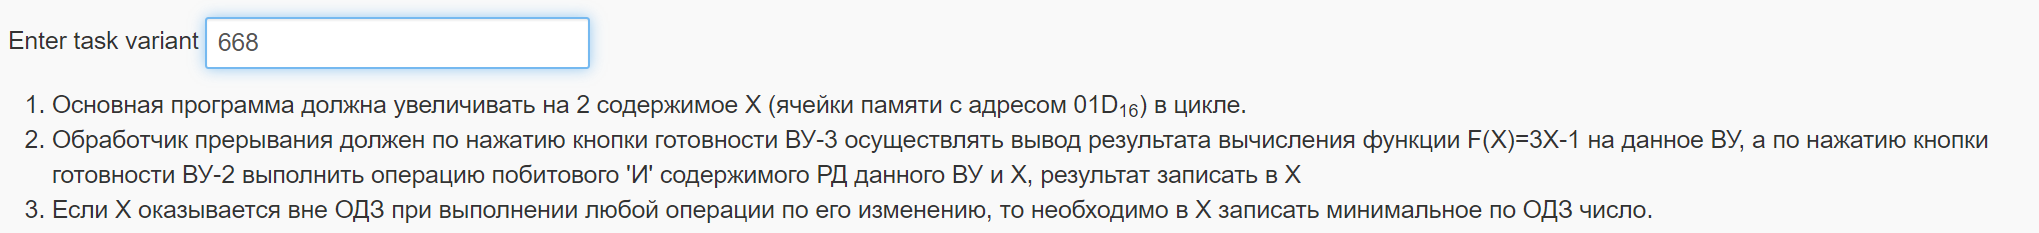
\includegraphics[scale=0.6]{task}
\label{pic:task}
\end{figure}

\section{Текст программы}
\begin{center}
\begin{tabular}{|c|c|c|l|}
\hline
\textbf{Адрес ячейки} & \textbf{Содержимое ячейки} & \textbf{Мнемоника} & \textbf{Комментарии}\\
\hline
58B & 05A1 & --- & Адрес начала массива\\
58C & 0200 & --- & Ячейка для хранения адреса \\
 & & & обрабатываемого элемента массива\\
58D & E000 & --- & Ячейка для хранения количества \\
 & & &необработанных элементов массива\\
58E & 0200 & --- & Ячейка для записи результата  \\ 
& & & работы программы\\
\hline
\hline
58F & 0200 & CLA & \\
590 & EEFD & ST (IP $-$ 3) & Загружаем 0 в ячейку 0x58E\\
\hline
591 & AF05 & LD \#0x5 & Помещаем количество элементов\\
592 & EEFA & ST (IP $-$ 6) & из аккумулятора в ячейку 0x58D\\
\hline
593 & 4EF7 & ADD (IP $-$ 9) & Помещаем адрес ячейки, следующей за\\
594 & EEF7 & ST (IP $-$ 9) & последним элементом массива в 0x58C\\
\hline
595 & ABF6 & LD $-$ (IP $-$ 10) & Автодекрементировав адрес ячейки в ячейке,\\
596 & F202 & BMI (IP $+$ 2) & загружаем текущий элемент массива\\
597 & 0300 & CLC & Если элемент меньше нуля, то формируем\\
598 & 0380 & CMC & бит переноса $ 0 $.\\
599 & 0200 & CLA & Если элемент больше нуля, то формируем\\
59A & 0280 & NOT & бит переноса $ 1 $.\\
59B & 2EF2 & AND (IP $-$ 14) & \\
59C & 0400 & ROL & Записываем результат анализа\\
59D & EEF0 & ST (IP $-$ 16) & в ячейку 0x58E\\
59E & 858D & LOOP 0x58D & Если остались необработанные\\
59F & CEF5 & BR (IP $-$ 11) & элементы, то переходим по адресу 0x595\\
5A0 & 0100 & HLT & Если нет, завершаем программу\\
\hline
\hline
5A1 & 759B & --- & \\
5A2 & 0500 & --- & \\
5A3 & F400 & --- & Элементы массива\\
5A4 & 0280 & --- & \\
5A5 & 459E & --- & \\
\hline
\end{tabular}
\end{center}



\section{Таблица трассировки}
\begin{center}
\begin{tabular}{|c|c|c|c|c|c|c|c|c|c|c|c|}
\hline
\multicolumn{2}{|c}{\makecell{\textbf{Выполняемая}\\\textbf{команда}}}
  &\multicolumn{8}{|c|}{\textbf{Содердимое регистров после выполнения команды}}
  &\multicolumn{2}{c|}{\makecell{\textbf{Ячейка, содержимое}\\\textbf{которой изменилось}}}\\
\hline
Адрес & Код & IP & CR & AR & DR & SP & BR & AC & NZVC & Адрес & Новый код\\
\hline
58F & 0200 & 590 & 0200 & 58F & 0200 & 000 & 058F & 0000 & 0100 & --- & ---\\
\hline
590 & EEFD & 591 & EEFD & 58E & 0000 & 000 & FFFD & 0000 & 0100 & 58E & 0000\\
\hline
591 & AF05 & 592 & AF05 & 591 & 0005 & 000 & 0005 & 0005 & 0000 & --- & ---\\
\hline
592 & EEFA & 593 & EEFA & 58D & 0005 & 000 & FFFA & 0005 & 0000 & 58D & 0005\\
\hline
593 & 4EF7 & 594 & 4EF7 & 58B & 05A1 & 000 & FFF7 & 05A6 & 0000 & --- & ---\\
\hline
594 & EEF7 & 595 & EEF7 & 58C & 05A6 & 000 & FFF7 & 05A6 & 0000 & 58C & 05A6\\
\hline
\hline
595 & ABF6 & 596 & ABF6 & 5A5 & 459E & 000 & FFF6 & 459E & 0000 & 58C & 05A5\\
\hline
596 & F202 & 597 & F202 & 596 & F202 & 000 & 0596 & 459E & 0000 & --- & ---\\
\hline
597 & 0300 & 598 & 0300 & 597 & 0300 & 000 & 0597 & 459E & 0000 & --- & ---\\
\hline
598 & 0380 & 599 & 0380 & 598 & 0380 & 000 & 0598 & 459E & 0001 & --- & ---\\
\hline
599 & 0200 & 59A & 0200 & 599 & 0200 & 000 & 0599 & 0000 & 0101 & --- & ---\\
\hline
59A & 0280 & 59B & 0280 & 59A & 0280 & 000 & 059A & FFFF & 1001 & --- & ---\\
\hline
59B & 2EF2 & 59C & 2EF2 & 58E & 0000 & 000 & FFF2 & 0000 & 0101 & --- & ---\\
\hline
59C & 0400 & 59D & 0400 & 59C & 0400 & 000 & 059C & 0001 & 0000 & --- & ---\\
\hline
59D & EEF0 & 59E & EEF0 & 58E & 0001 & 000 & FFF0 & 0001 & 0000 & 58E & 0001\\
\hline
59E & 858D & 59F & 858D & 58D & 0003 & 000 & 059E & 0001 & 0000 & 58D & 0004\\
\hline
59F & CEF5 & 595 & CEF5 & 59F & 595 & 000 & FFF5 & 0001 & 0000 & --- & ---\\
\hline
\hline
595 & ABF6 & 596 & ABF6 & 5A4 & 0280 & 000 & FFF6 & 0280 & 0000 & 58C & 05A4\\
\hline
596 & F202 & 597 & F202 & 596 & F202 & 000 & 0596 & 0280 & 0000 & --- & ---\\
\hline
597 & 0300 & 598 & 0300 & 597 & 0300 & 000 & 0597 & 0280 & 0000 & --- & ---\\
\hline
598 & 0380 & 599 & 0380 & 598 & 0380 & 000 & 0598 & 0280 & 0001 & --- & ---\\
\hline
599 & 0200 & 59A & 0200 & 599 & 0200 & 000 & 0599 & 0000 & 0101 & --- & ---\\
\hline
59A & 0280 & 59B & 0280 & 59A & 0280 & 000 & 059A & FFFF & 1001 & --- & ---\\
\hline
59B & 2EF2 & 59C & 2EF2 & 58E & 0001 & 000 & FFF2 & 0001 & 0001 & --- & ---\\
\hline
59C & 0400 & 59D & 0400 & 59C & 0400 & 000 & 059C & 0003 & 0000 & --- & ---\\
\hline
59D & EEF0 & 59E & EEF0 & 58E & 0003 & 000 & FFF0 & 0003 & 0000 & 58E & 0003\\
\hline
59E & 858D & 59F & 858D & 58D & 0002 & 000 & 059E & 0003 & 0000 & 58D & 0003\\
\hline
59F & CEF5 & 595 & CEF5 & 59F & 595 & 000 & FFF5 & 0003 & 0000 & --- & ---\\
\hline
\hline
595 & ABF6 & 596 & ABF6 & 5A3 & F400 & 000 & FFF6 & F400 & 1000 & 58C & 05A3\\
\hline
596 & F202 & 599 & F202 & 596 & F202 & 000 & 0002 & F400 & 1000 & --- & ---\\
\hline
599 & 0200 & 59A & 0200 & 599 & 0200 & 000 & 0599 & 0000 & 0100 & --- & ---\\
\hline
59A & 0280 & 59B & 0280 & 59A & 0280 & 000 & 059A & FFFF & 1000 & --- & ---\\
\hline
59B & 2EF2 & 59C & 2EF2 & 58E & 0003  & 000 & FFF2 & 0003 & 0000 & --- & ---\\
\hline
59C & 0400 & 59D & 0400 & 59C & 0400 & 000 & 059C & 0006 & 0000 & --- & ---\\
\hline
59D & EEF0 & 59E & EEF0 & 58E & 0006 & 000 & FFF0 & 0006 & 0000 & 58E & 0006\\
\hline
59E & 858D & 59F & 858D & 58D & 0001 & 000 & 059E & 0006 & 0000 & 58D & 0002\\
\hline
59F & CEF5 & 595 & CEF5 & 59F & 595 & 000 & FFF5 & 0006 & 0000 & --- & ---\\
\hline
\hline
595 & ABF6 & 596 & ABF6 & 5A2 & 0500 & 000 & FFF6 & 0500 & 0000 & 58C & 05A2\\
\hline
596 & F202 & 597 & F202 & 596 & F202 & 000 & 0596 & 0500 & 0000 & --- & ---\\
\hline
597 & 0300 & 598 & 0300 & 597 & 0300 & 000 & 0597 & 0500 & 0000 & --- & ---\\
\hline
598 & 0380 & 599 & 0380 & 598 & 0380 & 000 & 0598 & 0500 & 0001 & --- & ---\\
\hline
599 & 0200 & 59A & 0200 & 599 & 0200 & 000 & 0599 & 0000 & 0101 & --- & ---\\
\hline
59A & 0280 & 59B & 0280 & 59A & 0280 & 000 & 059A & FFFF & 1001 & --- & ---\\
\hline
59B & 2EF2 & 59C & 2EF2 & 58E & 0006 & 000 & FFF2 & 0006 & 0001 & --- & ---\\
\hline
59C & 0400 & 59D & 0400 & 59C & 0400 & 000 & 059C & 000D & 0000 & --- & ---\\
\hline
59D & EEF0 & 59E & EEF0 & 58E & 000D & 000 & FFF0 & 000D & 0000 & 58E & 000D\\
\hline
59E & 858D & 59E & 858D & 58D & 0000 & 000 & 059E & 000D & 0000 & 58D & 0001\\
\hline
59F & CEF5 & 595 & CEF5 & 59F & 595 & 000 & FFF5 & 000D & 0000 & --- & ---\\
\hline
\hline
595 & ABF6 & 596 & ABF6 & 5A1 & 759B & 000 & FFF6 & 759B & 0000 & 58C & 05A1\\
\hline
596 & F202 & 597 & F202 & 596 & F202 & 000 & 0596 & 759B & 0000 & --- & ---\\
\hline
597 & 0300 & 598 & 0300 & 597 & 0300 & 000 & 0597 & 759B & 0000 & --- & ---\\
\hline
598 & 0380 & 599 & 0380 & 598 & 0380 & 000 & 0598 & 759B & 0001 & --- & ---\\
\hline
599 & 0200 & 59A & 0200 & 599 & 0200 & 000 & 0599 & 0000 & 0101 & --- & ---\\
\hline
59A & 0280 & 59B & 0280 & 59A & 0280 & 000 & 059A & FFFF & 1001 & --- & ---\\
\hline
59B & 2EF2 & 59C & 2EF2 & 58E & 000D & 000 & FFF2 & 000D & 0001 & --- & ---\\
\hline
59C & 0400 & 59D & 0400 & 59C & 0400 & 000 & 059C & 001B & 0000 & --- & ---\\
\hline
59D & EEF0 & 59E & EEF0 & 58E & 001B & 000 & FFF0 & 001B & 0000 & 58E & 001B\\
\hline
59E & 858D & 59F & 858D & 58D & FFFF & 000 & 059E & 001B & 0000 & 58D & 0000\\
\hline
5A0 & 0100 & 5A1 & 0100 & 5A0 & 0100 & 000 & 5A0 & 001B & 0000 & --- & ---\\
\hline

\hline
\end{tabular}
\end{center}

\section{Описание программы}
\subsection{Предназначение}
Программа проходит каждый элемент массива с конца и исследует его элементы на знак (положительные/отрицательные). Если элемент является отрицательным, то программа оставляет флаг `C' равным 0, в противоположном случае делает флаг равным 1. Элементы массива в ходе исполнения программы не изменяются. Результат анализа записывается в ячейку 58E, причем перед записью результата анализа происходит сдвиг битов влево, поэтому один результат не будет перекрывать другой.

\subsection{Расположение программы в памяти}
\noindent Программа: 58F--5A0\\
Вспомогательные данные: 58B--58E\\
Элементы массива: 5A1--5A5

\subsection{Область представления}
\noindent Ячейки 5A1--5A5: 16-разрядные знаковые числа\\
Ячейки 58B, 58C: 11-разрядные беззнаковые числа\\
Ячейка 58D, 58E: 16-разрядное беззнаковое число\\


\subsection{Область допустимых значений}
\noindent Ячейки 5A1--5A5: $-2^{15}\ldots2^{15}-1$\\
Ячейки 58B, 58C: $0\ldots2^{11}$\\
Ячейка 58D, 58E: $0\ldots2^{16}$\\

\section{Вывод}
В ходе выполнения данной лабораторной работы я познакомился с режимами адресации БЭВМ и новыми для меня командами - ветвления, сравнения, командой LOOP. На практике разобрался с циклом выборки адреса дл разных режимов адресации.